% ============ CHAPTER 6 — DIGITAL TWIN WORLD ============
\chapter{The Digital Twin World}\label{cha:twin}

\section{World composition}

The twin is a full-scale, code-built 3~D world in Godot 4.7 running
(\texttt{godot/scenes/lts\_full.tscn}), with every geometric claim testable
in the 42-suite harness. Its composition:

\begin{figure}[H]
\centering
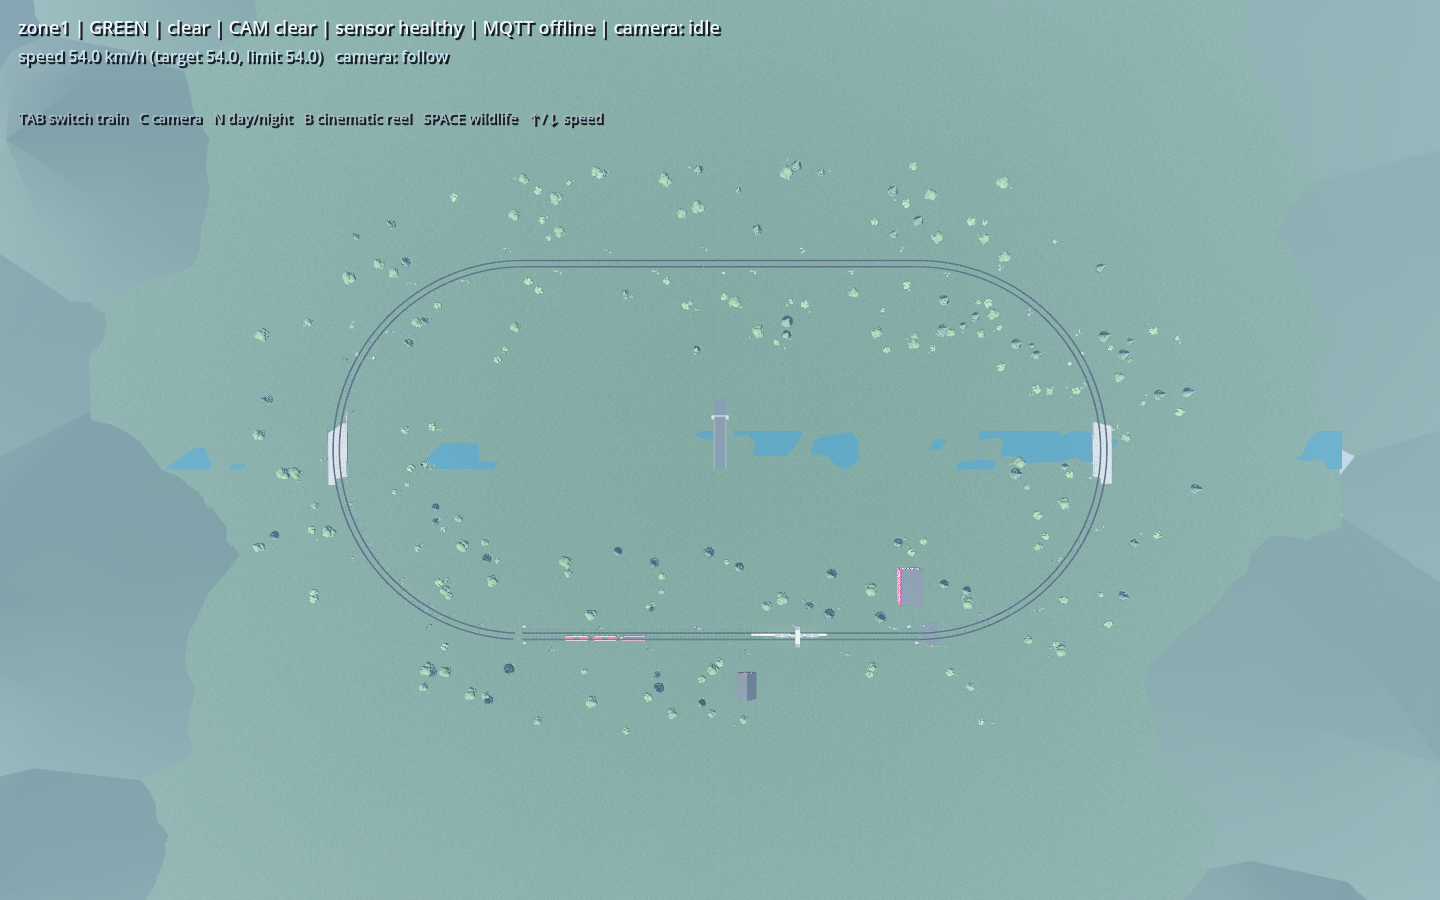
\includegraphics[width=16.8cm]{double_track_overview.png}
\caption{Top-down overview of the shared stadium footprint: UP and DOWN
tracks, the island station platform, carved river with a road and a railway
bridge, tree line, and the two-train fleet (HUD shows the active zone,
signal aspect, CAM state, sensor health, speed and camera mode). Captured
from \texttt{capture\_double\_track.gd} under headless software rendering;
the HUD \texttt{MQTT offline} flag is expected in capture mode where the
broker is intentionally not connected.}
\label{fig:overview}
\end{figure}

\begin{itemize}
  \item \textbf{Stadium double-track geometry:} UP and DOWN loops share a
        250\,m straight-sided stadium footprint --- centre lines
        \texttt{z = $\pm$120\,m}, straights \texttt{x = $-125..125$\,m},
        east/west curves of radius 120\,m. Closed lengths are UP
        1253.9822\,m and DOWN 1228.8495\,m, with block lengths 250.796\,m
        and 245.77\,m respectively (verified in \texttt{test\_stadium\_track}
        and \texttt{test\_geometry.test.js}).
  \item \textbf{Opposite running:} T1 runs clockwise on UP; T3 runs
        anticlockwise on DOWN with DOWN chainage converted
        (operational vs physical) and the opposite face---based on where
        the train is --- hidden from wildlife spawning logic
        (\texttt{test\_opposite\_running}).
  \item \textbf{Carved river and bridges:} a procedural river channel
        through the stadium with a road bridge and two widened railway
        bridge decks positioned at the track crossings; piers clear both
        rails and no tree is planted within 5\,m of either centre line
        (\texttt{test\_river\_bridges}, \texttt{test\_corridor\_flatten}).
  \item \textbf{Catenary and signals:} catenary wire runs above both
        lines; block signal masts display per-block aspects from the
        backend (\texttt{test\_catenary\_double},
        \texttt{test\_signal\_masts}).
\end{itemize}

\section{Island station and interlocked crossovers}

The island platform sits inside backend block UP-B2/DOWN-B2, built from
identical 9.6$\times$1.8$\times$2.2\,m modules with a canopy, benches and
bins (\texttt{test\_station\_island}); the platform spans chainage 150--198\,m
on the south straight.

\begin{figure}[H]
\centering
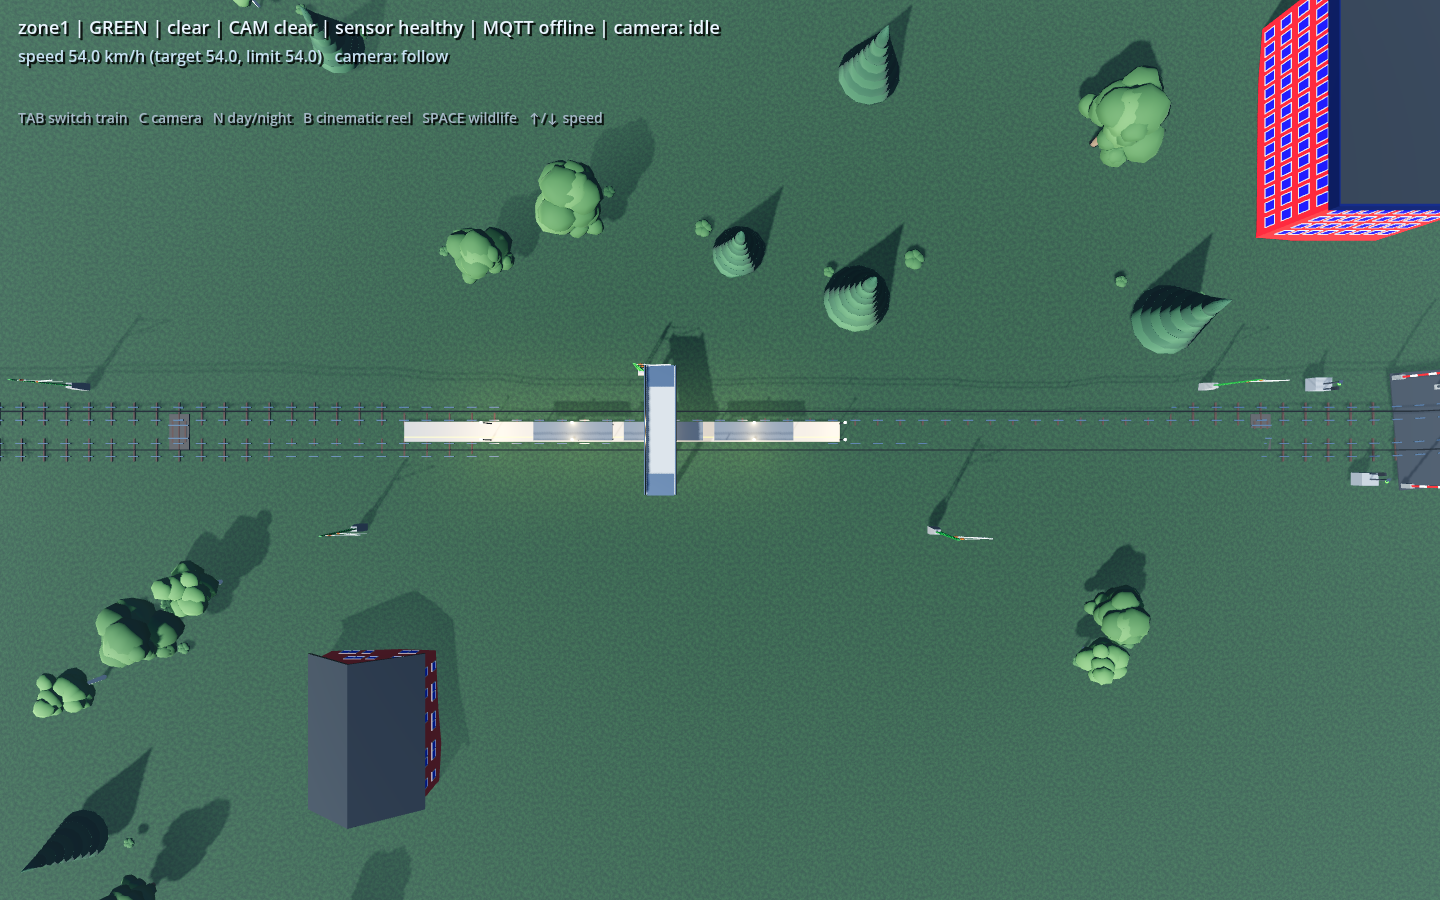
\includegraphics[width=16.8cm]{platform_after_topdown.png}
\caption{Island station from above: mainly-top view showing platform
modules, canopy/station building, both platforms and the two tracks.
Captured from \texttt{capture\_station.gd}.}
\label{fig:platform-topdown}
\end{figure}

\begin{figure}[H]
\centering
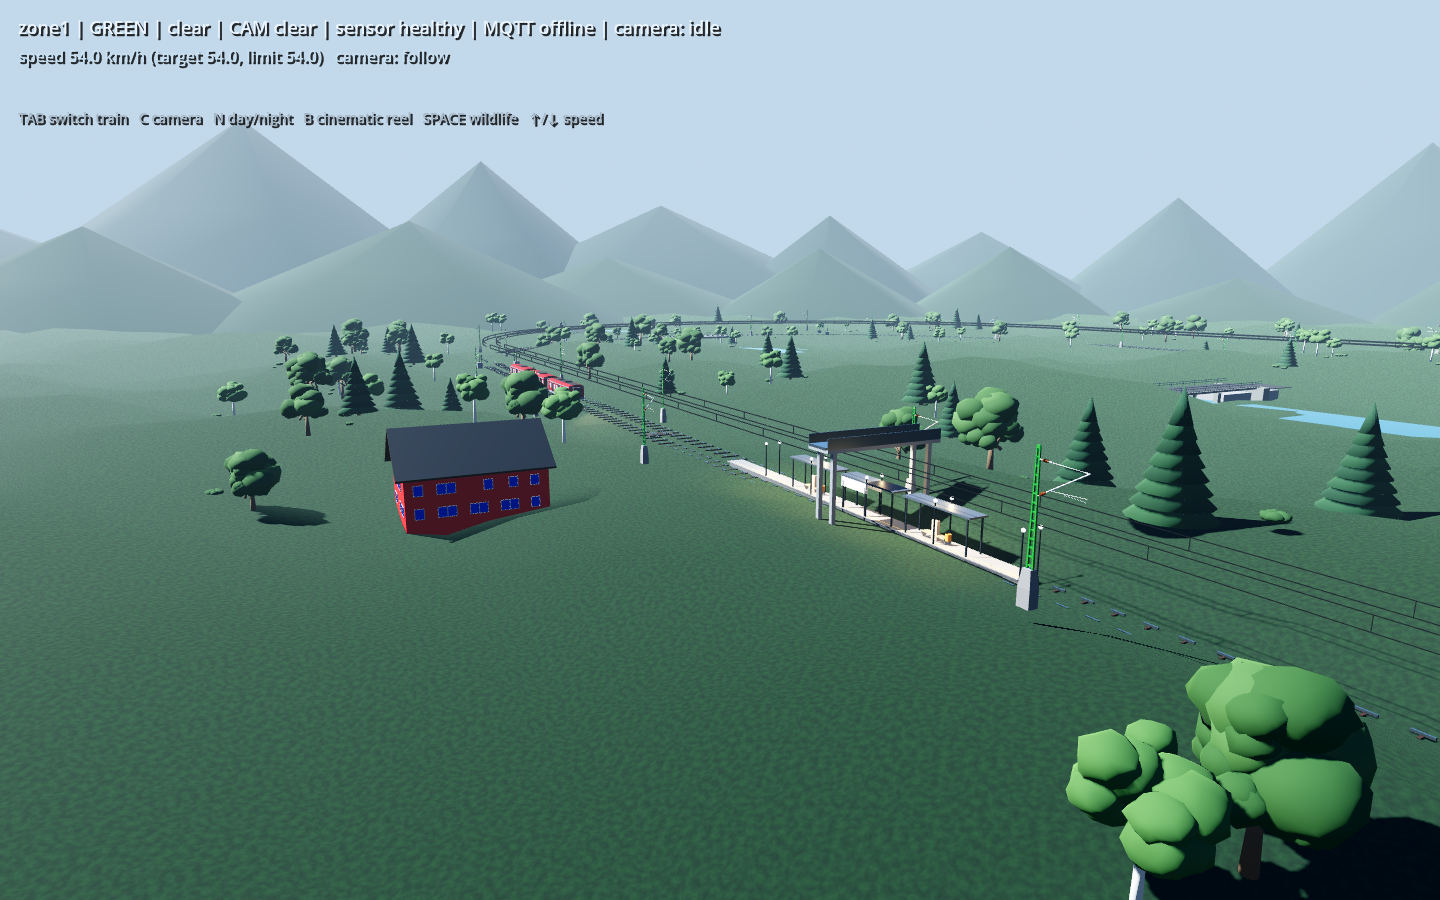
\includegraphics[width=16.8cm]{platform_after_oblique.png}
\caption{Island station at an oblique angle: platform modules and canopy
silhouette against \\ the parallel tracks and stadium corridor in the
background. Captured from \texttt{capture\_station.gd}.}
\label{fig:platform-oblique}
\end{figure}

Two station crossovers interlock the loops: \textbf{Crossover A} at UP
chainage 120\,m and \textbf{Crossover B} at UP chainage 240\,m, both ending
on both centre lines with visible switch blades
(\texttt{test\_station\_crossovers}). Routes are only granted through the
backend interlock (\texttt{routes.requestRoute}) and occupancy, hazard and
restrictive-zone checks are unchanged in every route type.

\section{Wrong-line run across the station}

An operator can request an interlocked wrong-line run: the requesting train
crosses from UP to DOWN at A, runs against traffic on the DOWN line, and
crosses back at B, while the opposing train is automatically held at a
point outside B inside braking distance.

\begin{figure}[H]
\centering
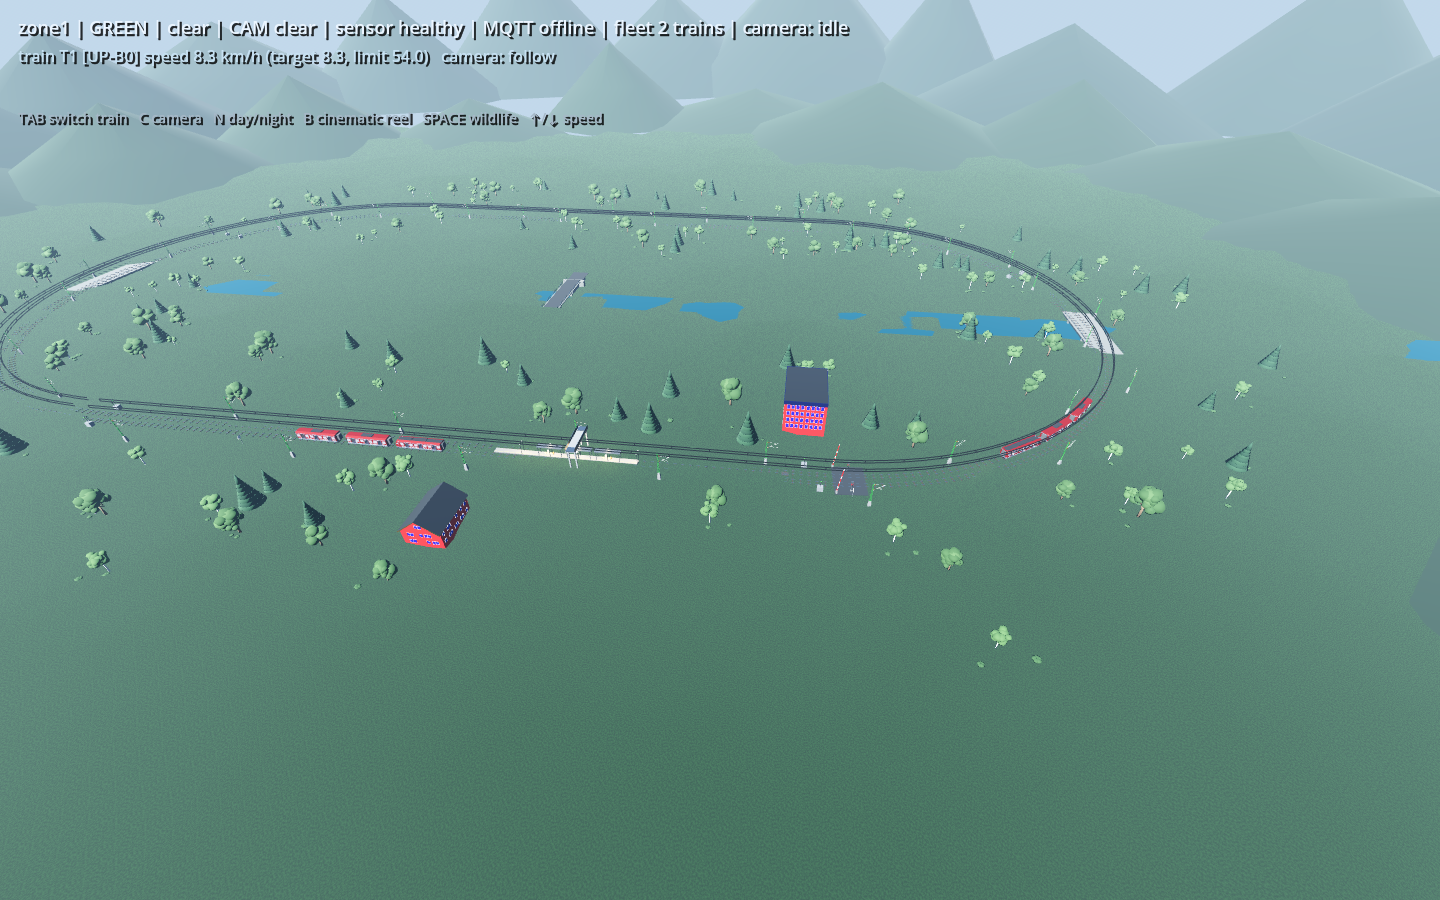
\includegraphics[width=16.2cm]{wrong_line_before.png}
\caption{Wrong-line run at UP phase APPROACH: T3 still on DOWN, T1
approaching crossover A before any visible motion; note HUD hold progress.
Captured from \texttt{capture\_crossover.gd}.}
\label{fig:wronglinebefore}
\end{figure}

\begin{figure}[H]
\centering
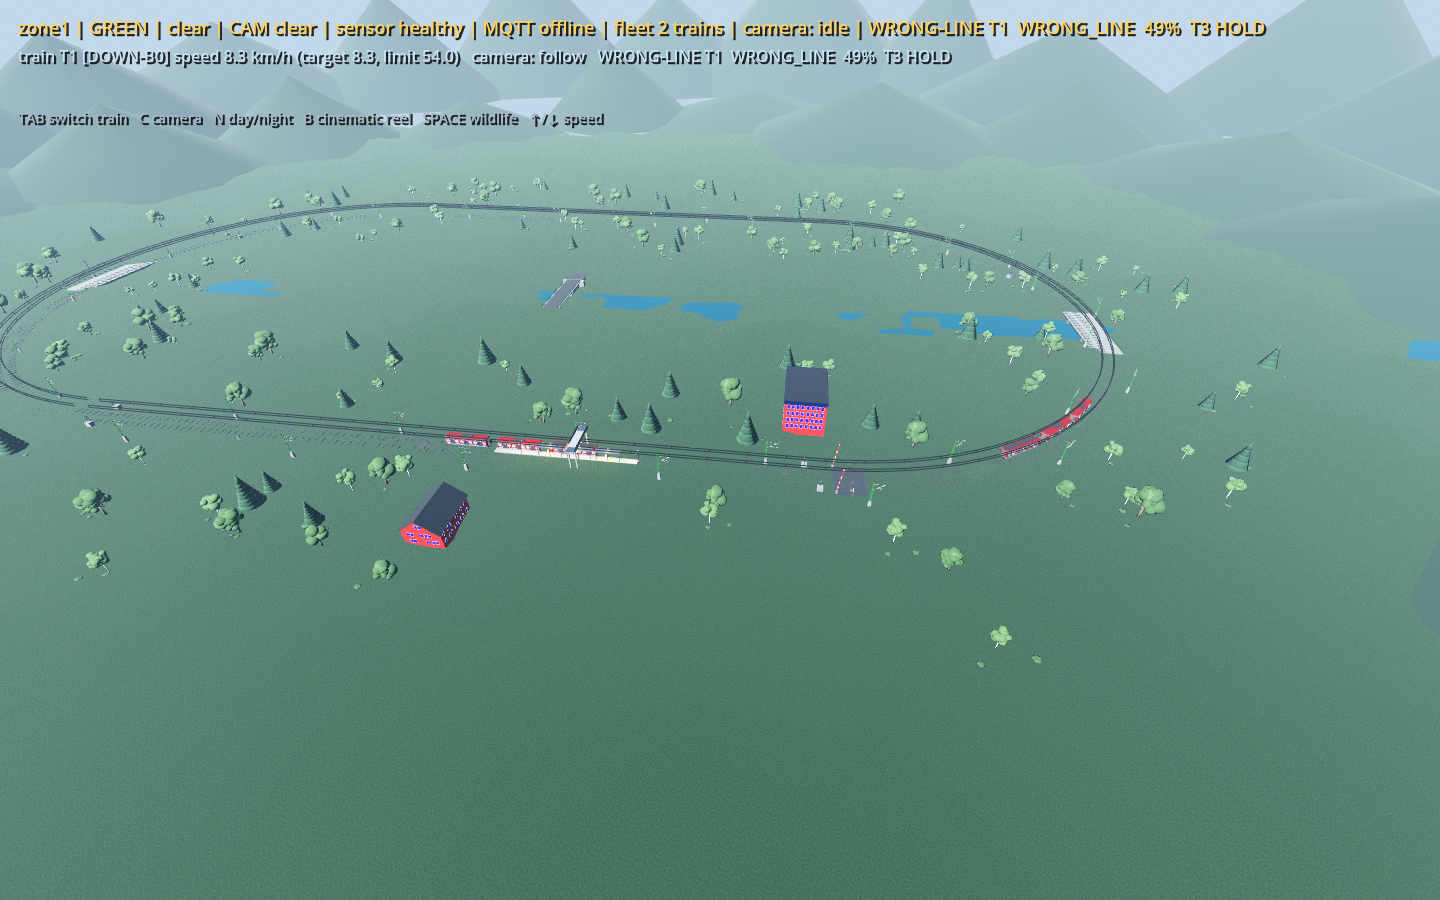
\includegraphics[width=16.2cm]{wrong_line_midway.png}
\caption{Wrong-line run at phase CROSS\_ENTRY/WRONG\_LINE: T1 blended onto
DOWN at A -- visible train between the switch points with switch blades in
motion. Captured from \texttt{capture\_crossover.gd}.}
\label{fig:wronglinemidway}
\end{figure}

\begin{figure}[H]
\centering
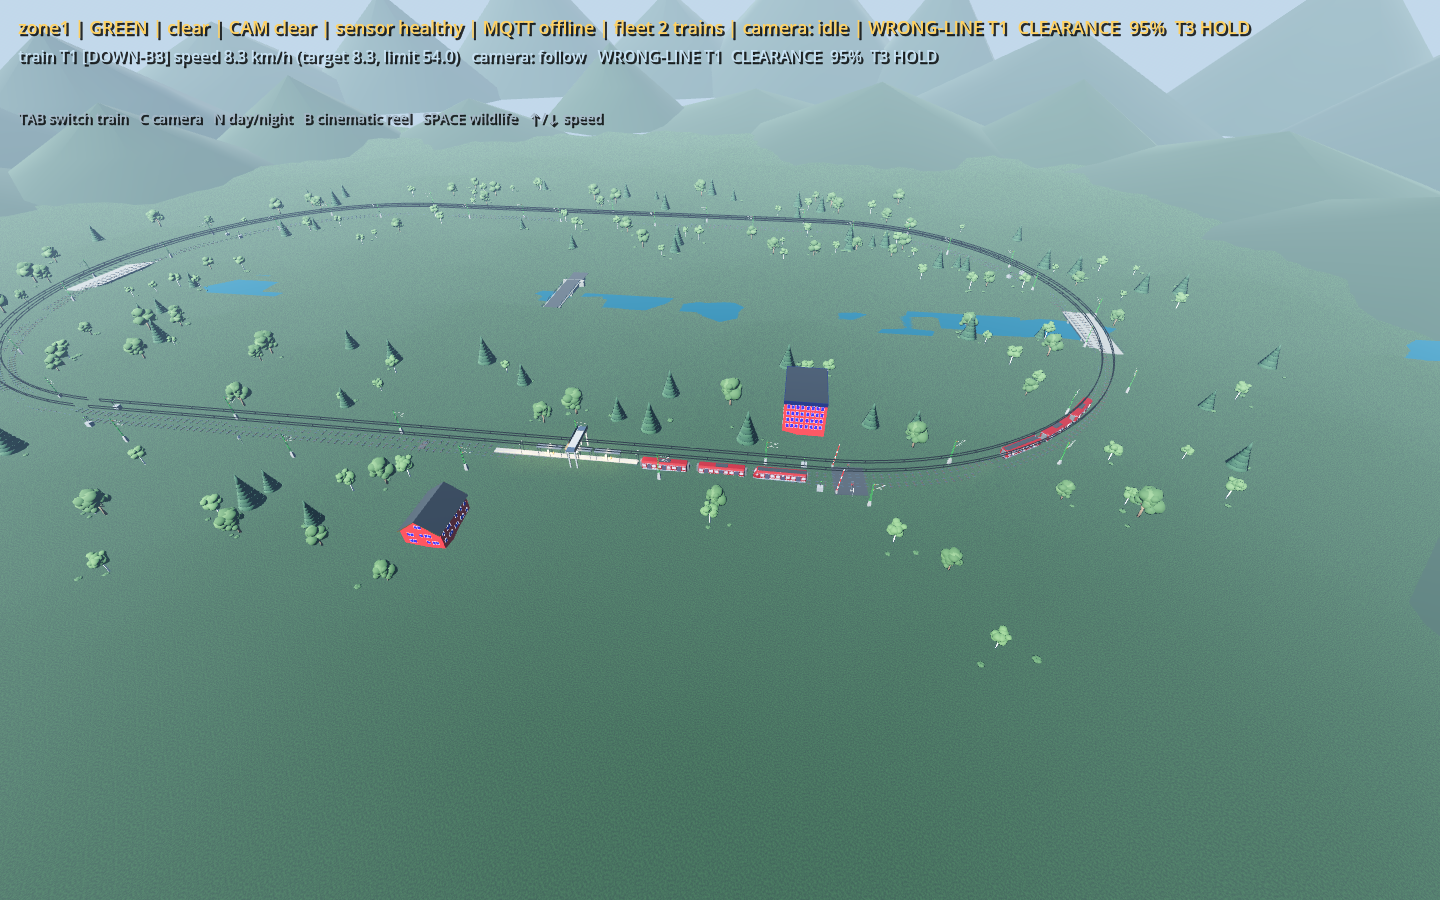
\includegraphics[width=16.2cm]{wrong_line_after.png}
\caption{Wrong-line run completion (phase CROSS\_EXIT/CLEARANCE): T1 back
on UP past B, T3 released from hold and both trains back under normal
authority. Captured from \texttt{capture\_crossover.gd}.}
\label{fig:wronglineafter}
\end{figure}

The visible crossover blend is backend-driven --- trains smoothly change
track without a snap; \texttt{test\_crossover\_visual} asserts smooth
movement across the join with no apply-state jump.

\section{Chance-based meets}

A seeded PRNG scheduled the meets the operator can trigger or let happen
naturally. A trigger window holds one of the two trains at the station
with \texttt{commandedSpeedKmh=0} at the backend so the meet only happens
when the other train is near; completion uses a proper interlocked
crossover route.

\begin{figure}[H]
\centering
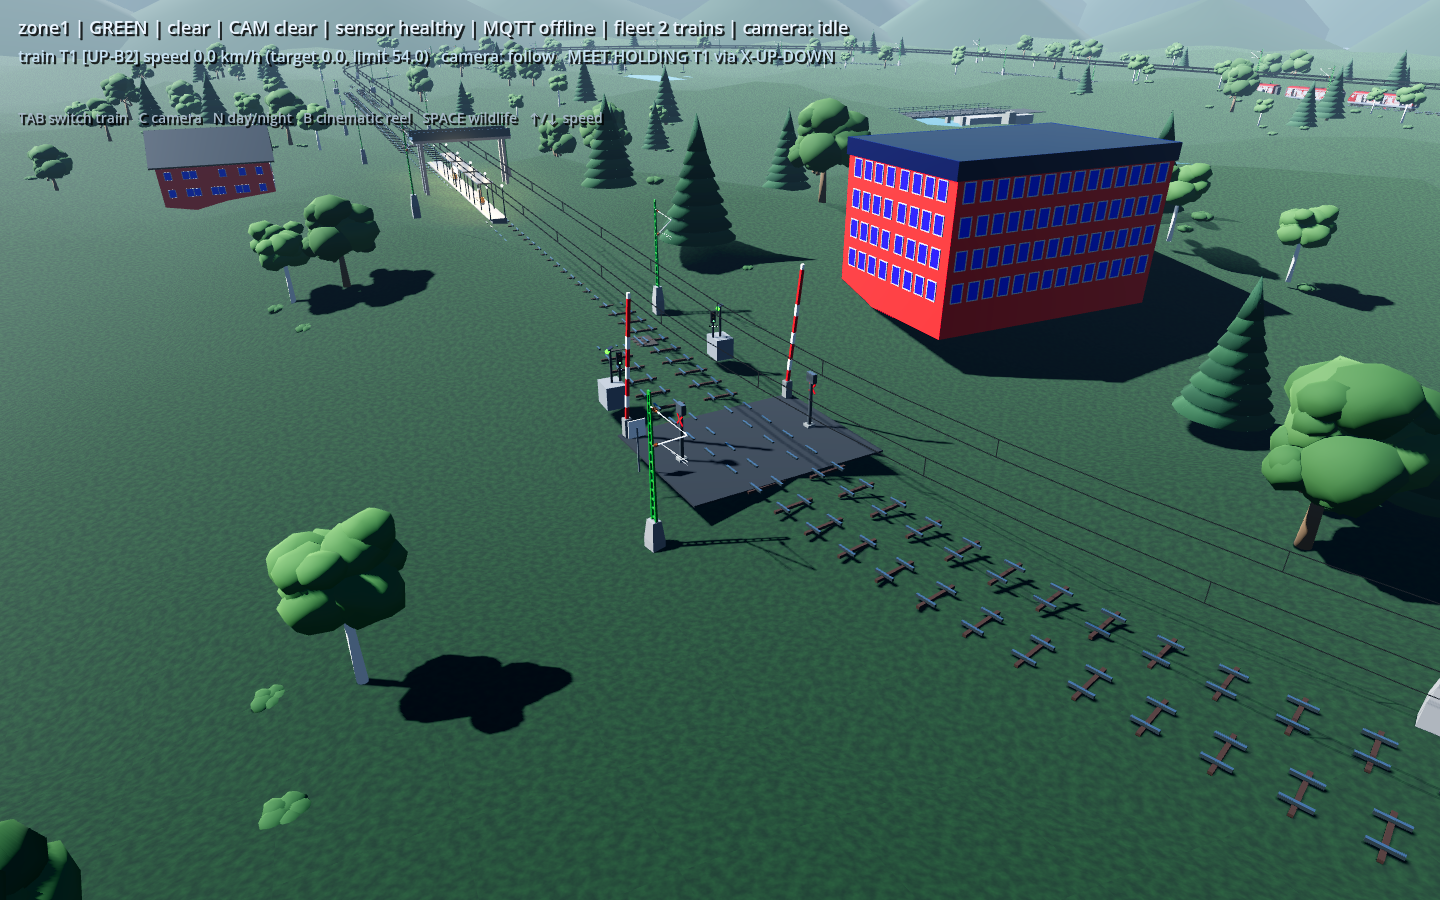
\includegraphics[width=16.8cm]{meet_randomized.png}
\caption{Live meet execution with seed 4242: both trains near the island
platform, one held, with the meet HUD showing phase, holder, chosen route
and countdown. Captured from \texttt{capture\_meet.gd}.}
\label{fig:meet}
\end{figure}

\section{The LTS asset fleet}

The twin replaces procedural stubs with real \textbf{Libre-TrainSim}
(LTS) exports: the train consist GLBs (cab car and
coaches), the island station modules, plus deer and elephant animals with
articulated limbs (verified by \texttt{test\_real\_assets}, which checks
the GLBs have landed in the scene graph and are placed on the correct
track). \texttt{tools/export\_lts\_assets.py} / \texttt{.sh} convert the
LTS Blender source files; \texttt{godot/assets.manifest.json} records
asset provenance and paths.

\begin{figure}[H]
\centering
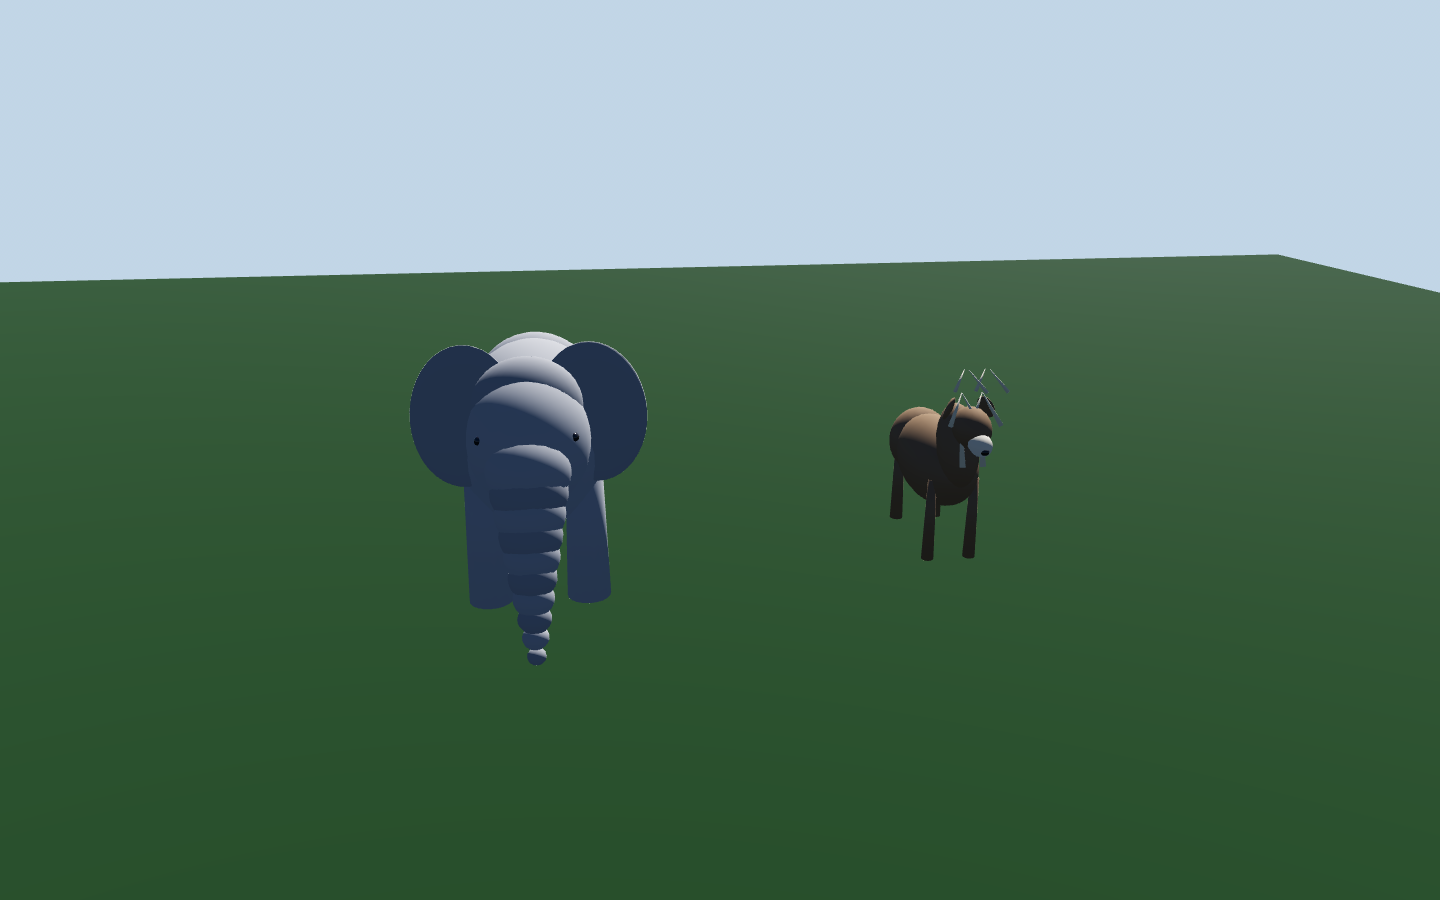
\includegraphics[width=16.2cm]{animals_scene.png}
\caption{Wokwi-style animal-assets sanity render: deer and elephant GLBs
with articulated limbs posed near the track, plus the sensor hut and
barrier kit. Captured from \texttt{capture\_animals.gd}.}
\label{fig:animals}
\end{figure}

Figure~\ref{fig:cameraconfirm} (Chapter~\ref{cha:dashboards}) shows the
same fleet in the live safety chain confirmed elephant ahead at 0.95/
confidence with a STOP already applied by the twin.

\section{Operator and observer surfaces of the twin}

\begin{itemize}
  \item \textbf{Keyboard:} \texttt{SPACE} toggles a zone-1 wildlife event,
        \texttt{F} toggles the sensor fault, \texttt{R} resets (only with
        all clear), \texttt{Up/Down} adjust local target speed
        (8\,km/h steps), \texttt{2} toggles zone-2 wildlife,
        \texttt{C} cycles camera modes (four modes, incl.\ orbit and
        onboard), \texttt{N} day/night.
  \item \textbf{HUD:} a debug bar continuously reports zone state, signal,
        CAM/HUT evidence path, sensor health, backend connection,
        camera status and speed; fleet-level HUD adds per-train lines, and
        the wrong-line HUD shows phase and percentage progress plus the
        opposing train hold state (\texttt{test\_wrong\_line\_hud}).
  \item \textbf{Camera director:} choose mode with \texttt{C}; capture
        scripts reuse the same director for deterministic angles used in
        the gates and in this report.
\end{itemize}

\section{Twin subsystem modules}

\begin{longtable}{>{\raggedright}p{4.0cm} >{\raggedright\arraybackslash}p{11.6cm}}
\caption{Key \texttt{godot/src} modules}\label{tab:twinmodules}\\
\toprule
\textbf{Module} & \textbf{Responsibility} \\
\midrule
\endfirsthead
\caption[]{(continued)}\\
\toprule
\textbf{Module} & \textbf{Responsibility} \\
\midrule
\endhead
\texttt{mqtt\_bridge.gd} & MQTT inbound/outbound with exponential backoff on broker failure \\
\texttt{train\_reconciler.gd} / \texttt{fleet\_controller.gd} & Apply authoritative backend state to the twin fleet (speeds, signals, routes) \\
\texttt{track\_registry.gd} / \texttt{ltstrack.gd} / \texttt{track\_builder.gd} & Stadium track geometry, chainage conversion, mesh building \\
\texttt{level\_crossing.gd} & Two-track level crossing: alarms, pivoting booms, light logic \\
\texttt{wildlife\_director.gd} / \texttt{wildlife\_spawner.gd} & Deterministic seeded wildlife appearances at correct chainage and distance \\
\texttt{wildlife\_safety.gd} / \texttt{animal\_safety\_system.gd} & Local fail-safe layers with backend precedence logic \\
\texttt{onboard\_braking.gd} / \texttt{detection\_band.gd} & Quadratic stopping-distance and safe-speed inversion \\
\texttt{animal\_detector.gd} / \texttt{camera\_confirmation.gd} & Simulated forward camera (cone, occlusion) and evidence upload \\
\texttt{trackside\_sensor\_hut.gd} / \texttt{wildlife\_sensor\_network.gd} & Distributed hut observations \\
\texttt{block\_signal\_mast.gd} / \texttt{safety\_signals.gd} & Visual per-block aspects \\
\texttt{camera\_director.gd} / \texttt{twin\_hud.gd} & Cameras and the HUD overlaid in captures \\
\bottomrule
\end{longtable}
